 \thispagestyle{gocconone}
\pagestyle{gocco}
\everymath{\color{gocco}}
\graphicspath{{../gocco/pic/}}
\blfootnote{$^1${\color[named]{gocco}Trung tâm Quy hoạch và Điều tra tài nguyên -- môi trường biển khu vực phía Nam.}}
\begingroup
\AddToShipoutPicture*{\put(0,616){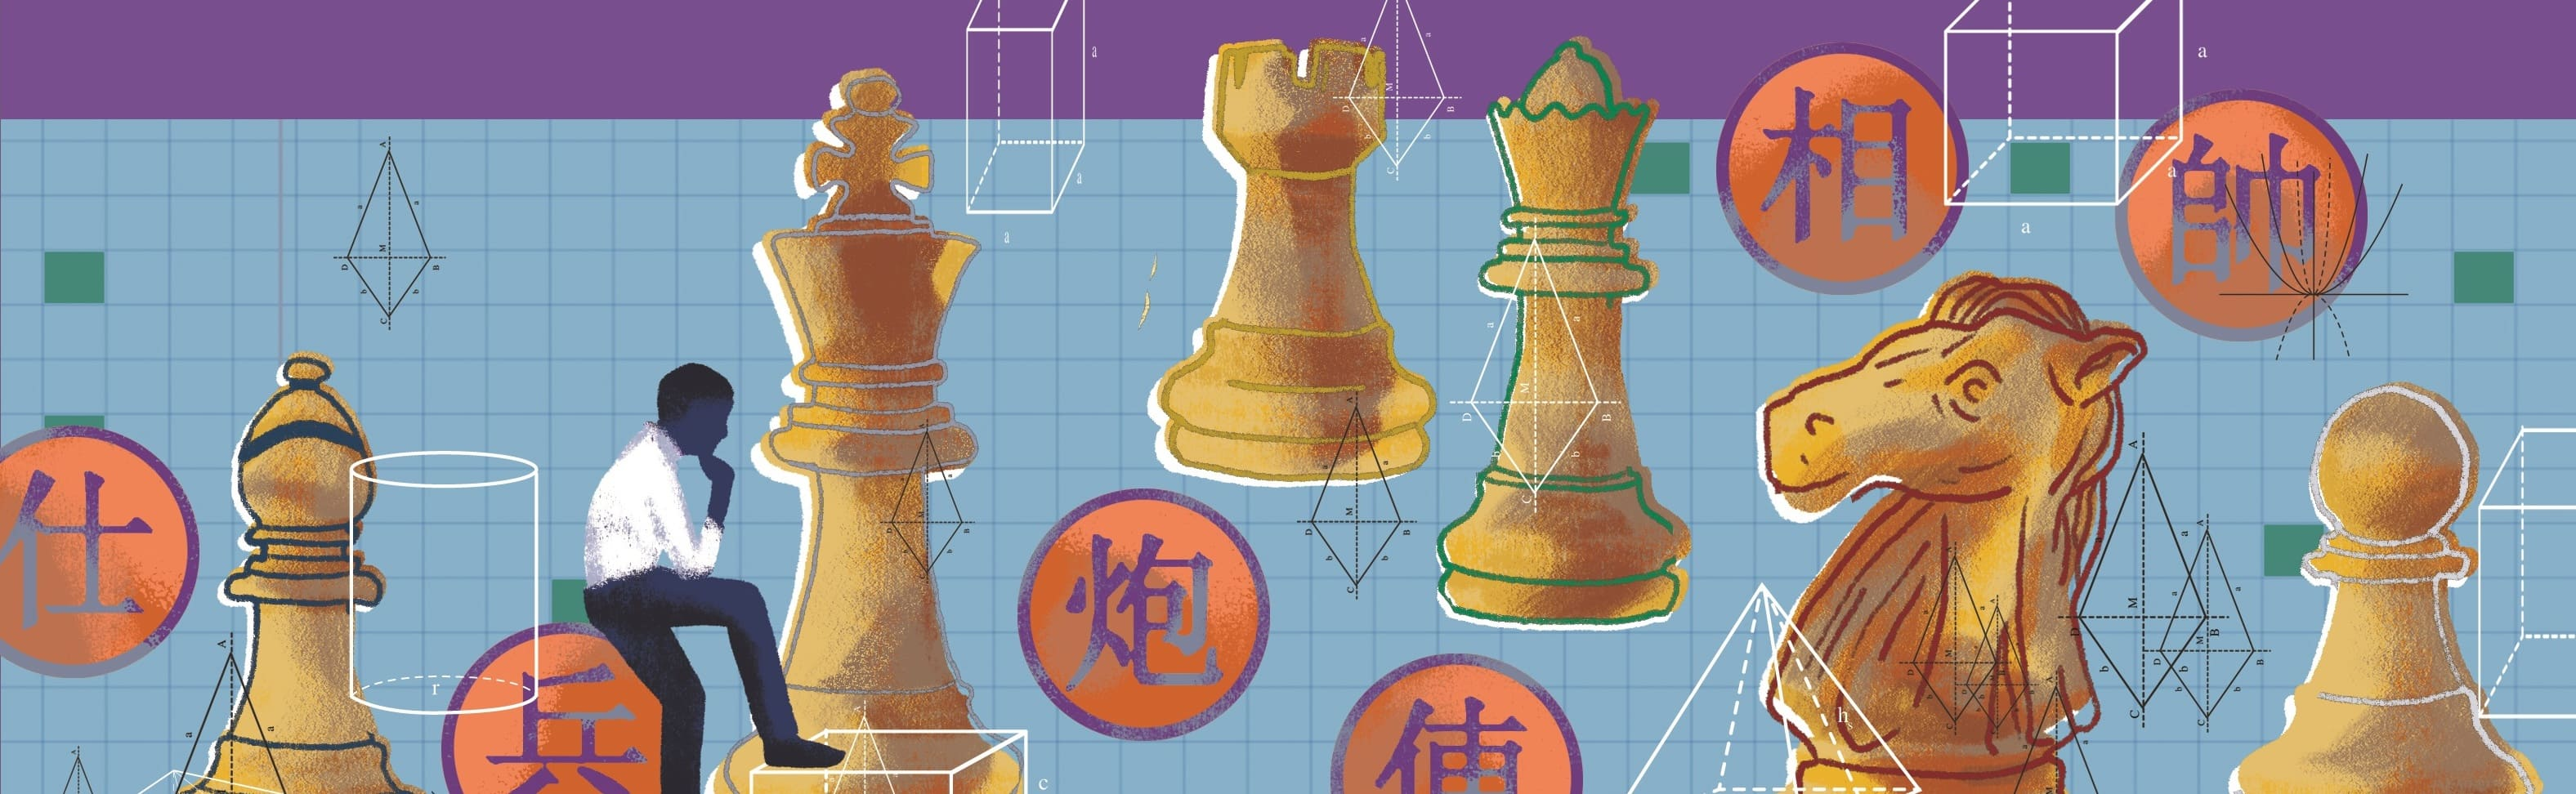
\includegraphics[width=19.3cm]{../bannergocco}}}
\AddToShipoutPicture*{\put(141,550){
\includegraphics[scale=1]{../tieude2.pdf}}} 
\centering
\endgroup

\vspace*{160pt}
\begin{multicols}{2}
	Tàn cuộc Pháo--Mã--Chốt, thường được gọi với những cái tên khác như: Cờ tàn không Xe hay cờ tàn đi bộ ... Đó là loại hình tàn cuộc rất thường hay gặp trong thực chiến. Lúc này ván đấu đã đi đến giai đoạn cuối cùng, đôi bên đã đổi hết $2$ quân Xe chủ lực, và đây chính là thời điểm các kỳ thủ cần phải vận dụng hết nội lực cờ tàn, đặc biệt là kỹ năng sử dụng những quân ``nhẹ" nhằm giành lấy  kết quả có lợi nhất.
	\vskip 0.1cm
	Tuy nhiên, đối với các kỳ thủ nghiệp dư, chưa có nhiều kinh nghiệm và kiến thức về cờ Tàn thường cảm thầy rằng Pháo Mã Chốt rất khó sử dụng nếu thiếu đi quân Xe trợ chiến. Vì lẽ đó, khi đối diện với những hình cờ không Xe thường gặp không ít lúng túng, điều quân thiếu kế hoạch làm cục diện trở nên rối ren và phức tạp hơn, đi những nước đi tự làm khó, bỏ qua những cơ hội chiến thắng, thậm chí còn có thể để thua trong những tình huống hòa cơ bản.
	\vskip 0.1cm
	Ngày nay, trình độ chung của các kỳ thủ ngày càng được cải thiện, những cuộc chiến đỉnh cao xuất hiện càng nhiều, tàn cuộc không xe lại càng đóng vai trò quan trọng hơn bao giờ hết. Để xử lý tốt loại hình này, đòi hỏi các kỳ thủ phải có nền móng kiến thức cờ tàn thật sự vững chắc, đồng thời cũng cần sở hữu kỹ năng điều động các quân khéo léo và uyển chuyển, nhạy bén trong nghệ thuật chuyển đổi hình trận.
	\vskip 0.1cm
	Trong bài viết kỳ này, tác giả sẽ gửi đến bạn đọc Pi những ván cờ tàn sử dụng những nước đi Pháo Mã Chốt đặc sắc. Mong rằng sau những ví dụ này, bạn đọc sẽ rút ra được những kinh nghiệm bổ ích khi xử lý những hình cờ tàn không Xe, một trong những vẻ đẹp của nghệ thuật Tượng Kỳ.
	\begin{figure}[H]
		\centering
		\vspace*{-5pt}
		\captionsetup{labelformat= empty, justification=centering}
		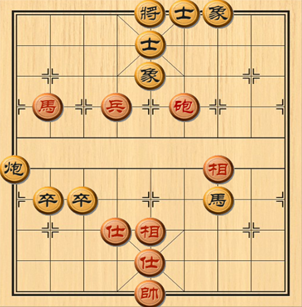
\includegraphics[width=0.4\textwidth]{1}
		\caption{\small\textit{\color{gocco}Hình $1$.}}
		\vspace*{-10pt}
	\end{figure}
	$1.$ Hình $1$, nhìn qua có vẻ như hình cờ đang cân bằng, Đôi bên đều còn Pháo Mã Chốt và đầy đủ Sỹ Tượng. Thậm chí Đen có lợi thế hơn vì hơn $1$ Chốt qua sông và hệ thống Sỹ Tượng của Đỏ ở vị trí không ổn định. Nhưng Đỏ được quyền đi trước và tung ra những đòn đánh để kết thúc ván cờ như sau:
	\vskip 0.1cm
	$\pmb{1)}$ M$8.7$ Tg$-4$\quad $\pmb{2)}$ P$4/1$ Tg$.1$$(*)$\quad $\pmb{3)}$ P$4-6$ S$5.4$\quad $\pmb{4)}$ C$6.1$ Tg$-5$\quad $\pmb{5)}$ P$6-8$ Tg$-6$$(**)$\quad $\pmb{6)}$ C$6-5$ S$6.5$\quad $\pmb{7)}$ M$7/6$ S$5.4$\quad $\pmb{8)}$ P$8-4$ ($1-0$)
	\vskip 0.1cm
	\textit{$(*)$: Nhận thấy các quân đang ở vị trí thuận lợi Đỏ ngay lập tức có $2$ nước liên tục điều quân đến vị trí thuận lợi, trước tấn Mã chiếu ngọa tào, sau thoái Pháo dọa sát. Do đó, bắt buộc Đen phải di chuyển  Tướng đến vị trí kém an toàn.
	\vskip 0.1cm
	$(**)$: Liên tục là những nước quấy rối và dọa sát của Đỏ, tạo điều kiện cho quân Chốt ngang nhiên áp sát trận địa, bẻ bớt Sỹ Tượng nhưng Đen chỉ biết chống trả một cách bị động. Thắng lợi giành cho Đỏ chỉ còn là vấn đề thời gian. }
	\begin{figure}[H]
		\centering
		\vspace*{-5pt}
		\captionsetup{labelformat= empty, justification=centering}
		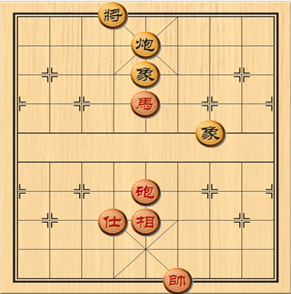
\includegraphics[width=0.4\textwidth]{2}
		\caption{\small\textit{\color{gocco}Hình $2$.}}
		\vspace*{-10pt}
	\end{figure}
	$2$. Hình $2$, đây là một trong những dạng căn bản của cờ tàn Pháo, Mã. Đỏ đang có lợi thế khi hơn $1$ quân chủ lực. Tuy nhiên. Bên Đen còn Pháo và song Tượng phòng thủ cũng rất dẻo dai, nếu bên cầm Đỏ thiếu kinh nghiệm sẽ không dễ gì giành chiến thắng. Đỏ cần phải chơi như sau:
	\vskip 0.1cm 
	$\pmb{1)}$	M$5.7$ P$5-3$$(*)$\quad $\pmb{2)}$ P$5.3$ T$g.1$\quad $\pmb{3)}$ T$5.3$ T$5.3$\quad  $\pmb{4)}$ P$5-4$ T$3/5$\quad $\pmb{5)}$ Tg$4-5$$(**)$ T$7/9$\quad $\pmb{6)}$ P$4/5$ Tg$/1$\quad $\pmb{7)}$P$4-7$ T$5.7$\quad $\pmb{8)}$ P$7-6$$(***)$ ($1-0$)
	\vskip 0.1cm
	\textit{$(*)$: Tấn Mã vừa chiếu Tướng, vừa dùng Pháo bắt Mã một nước đi cần thiết để khóa quân đối phương, để tránh mất quân, Đen phải bình Pháo cản Mã Đỏ.
	\vskip 0.1cm
	$(**)$ Liên tiếp là những nước đi rất có ý đồ của Đỏ, nhằm dùng mặt Tướng chiếm lấy trung lộ, chuẩn bị thoái Pháo phối hợp với Sỹ để lấy mạng tướng đối phương.
	\vskip 0.1cm
	$(***)$: Đỏ thoái pháo về cung Tướng, vừa dọa P$4-6$ sát cục lại vừa có thể đi P$4-7$ khi cần thiết. 
	\vskip 0.1cm
	Nhìn chung, với dạng cờ tàn này, Mã tấn công tầm gần còn Pháo uy hiếp tầm xa; $2$ quân này sẽ luân phiên đổi vai trò cho nhau, Mã khống chế thì Pháo sẽ là quân tìm cách chiếu hết và ngược lại.}
	\begin{figure}[H]
		\centering
		\vspace*{-5pt}
		\captionsetup{labelformat= empty, justification=centering}
		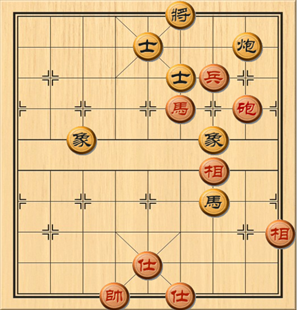
\includegraphics[width=0.4\textwidth]{3}
		\caption{\small\textit{\color{gocco}Hình $3$.}}
		\vspace*{-10pt}
	\end{figure}
	$3.$ Hình $3$, đôi bên đang có quân lực khá đồng đều, nhưng chỉ cần ưu thế $1$ Chốt và $3$ quân tấn công đang tập trung bên cánh phải, Đỏ đã kết thúc ván đấu như sau:
	\vskip 0.1cm
	$\pmb{1)}$ C$3.1$$(*)$ M$7/9$\quad $\pmb{2)}$ P$2.1$ P$8-9$\quad $\pmb{3)}$ P$2.2$ Tg$-5$$(**)$\quad $\pmb{4)}$ M$4.2$ P$9.2$\quad $\pmb{5)}$ C$3-4$ P$9-8$\quad $\pmb{6)}$ M$2.3$$(***)$  S$5/6$\quad $\pmb{7)}$ P$2-1$ P$8/3$\quad $\pmb{8)}$ M$3/4$ T$3/1$\quad $\pmb{9)}$ P$1/1$$(****)$ ($1-0$)
	\vskip 0.1cm
	\textit{$(*)$: Nhận thấy Pháo Đen đang ở vị trí khá xấu, Đỏ ngay lập tức tấn Chốt chiếm tiên thủ, cũng vừa để áp sát cung Tướng đối phương.
	\vskip 0.1cm
	$(**)$: Ý muốn đổi quân cầu hòa của Đen được bộc lộ rất rõ ở nước M$7/9$, tất nhiên Đỏ không dễ gì chấp nhận điều đó. Sau khi tấn Pháo ép buộc Pháo Đen phải né tránh, Đỏ ngay lập tức tấn Pháo xuống tuyến đáy, đe dọa sát cuộc ngay lập tức.
	\vskip 0.1cm
	$(***)$: Sau một loạt nước điều quân, hệ thống Pháo Mã Chốt của Đỏ đã tập trung tại vị trí đắc địa, sẵn sàng lấy mạng Tướng địch bất cứ lúc nào.
	\vskip 0.1cm
	$(****)$: Mặc dù Đen rất tích cực trong việc phòng thủ, hết thoái Sỹ rồi lùi Pháo về làm dày tuyến đáy nhưng đều vô ích. Sau khi Đỏ đi P1/1, Đen nhìn thấy trước nước bình Chốt sát cục nhưng không có cách nào phòng thủ, Đen chấp nhận đầu hàng.}
	\vskip 0.1cm
	\textit{Chú thích}: C: Chốt, X: Xe, M: Mã, P: Pháo, Tg: Tướng, S: Sỹ, T: Tượng, s: Sau.
	\vskip 0.1cm
	\textbf{\color{gocco}Câu đố kỳ này}
	\vskip 0.1cm
	Cả $2$ hình cờ dưới đây đều có đặc điểm là Đỏ đều hơn $1$ quân chủ lực, đôi bên đều còn đầy đủ Sỹ Tượng, điểm khác biệt duy nhất là tại hình $4$ Đen còn Pháo và hình $5$ còn Mã. Chính sự khác biệt này tạo ra kết quả khác biệt. Câu hỏi đặt ra là, nếu đôi bên đi những nước đi chính xác, hình nào bên Đỏ giành chiến thắng và hình nào có kết quả hòa ?
	\begin{figure}[H]
		\centering
		\vspace*{-5pt}
		\captionsetup{labelformat= empty, justification=centering}
		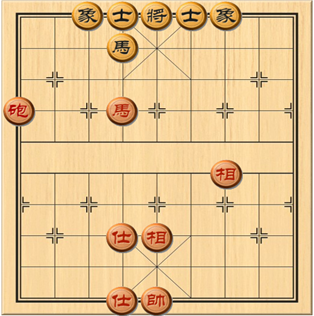
\includegraphics[width=0.4\textwidth]{4}
		\caption{\small\textit{\color{gocco}Hình $4$.}}
		\vspace*{-10pt}
	\end{figure}
	\begin{figure}[H]
		\centering
		\vspace*{5pt}
		\captionsetup{labelformat= empty, justification=centering}
		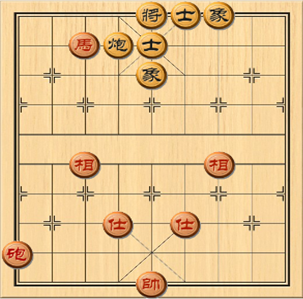
\includegraphics[width=0.4\textwidth]{5}
		\caption{\small\textit{\color{gocco}Hình $5$.}}
		\vspace*{-10pt}
	\end{figure}
	\textit{Đáp án:}
	Đối với những ai có một chút kiến thức về cờ tàn căn bản thì sẽ không mấy khó khăn để tìm ra đáp án trong $2$ hình cờ trên. Nếu đôi bên đi chính xác thì Hình $4$ sẽ có kết quả thắng và Hình $5$ có kết quả hòa, cụ thể như sau: 
	\vskip 0.1cm
	Hình $4$: $\pmb{1)}$ M$6.7$ S$4.5$\quad $2)$ P$9/5$ S$5.4$\quad $3)$ P$9-3$ T$7.9$\quad $4)$ P$3-6$ S$6.5$\quad $5)$ T$5/3$ Tg$-4$\quad $\pmb{6)}$ P$6-7$ T$3.1$ \quad $\pmb{7)}$ M$7/9$. Đen mất Tượng chắc chắn thua cuộc ($1-0$).
	\vskip 0.1cm
	Hình $5$: $\pmb{1)}$ M$7/8$ S$5.6$\quad $\pmb{2)}$ T$7/5$ S$s.5$\quad $\pmb{3)}$ S$6/5$ P$4.5$\quad $\pmb{4)}$ P$9.4$ P$4-8$\quad $\pmb{5)}$ M$8.7$ Tg$-4$\quad $\pmb{6)}$ P$9-5$ P$8/3$\quad $\pmb{7)}$ M$7/6$ P$8/2$\quad $\pmb{8)}$ T$5/7$ T$5/3$\quad $\pmb{9)}$ T$3/5$ P$8-6$\quad $\pmb{10)}$ M$6/8$ T$3.5$\quad $\pmb{11)}$ M$8.6$ P$6-7$\quad $\pmb{12)}$ P$5-6$ Tg$-5$\quad $\pmb{13)}$ P$6-4$ T$5/3$. Mặc dù Đỏ hơn quân nhưng Đen phòng thủ vô cùng chắc chắn, hòa cuộc ($1/2$).
\end{multicols}




